\subsection{Dense Layer}

\subsubsection{Operation}
\begin{figure}[h]
	\centering
	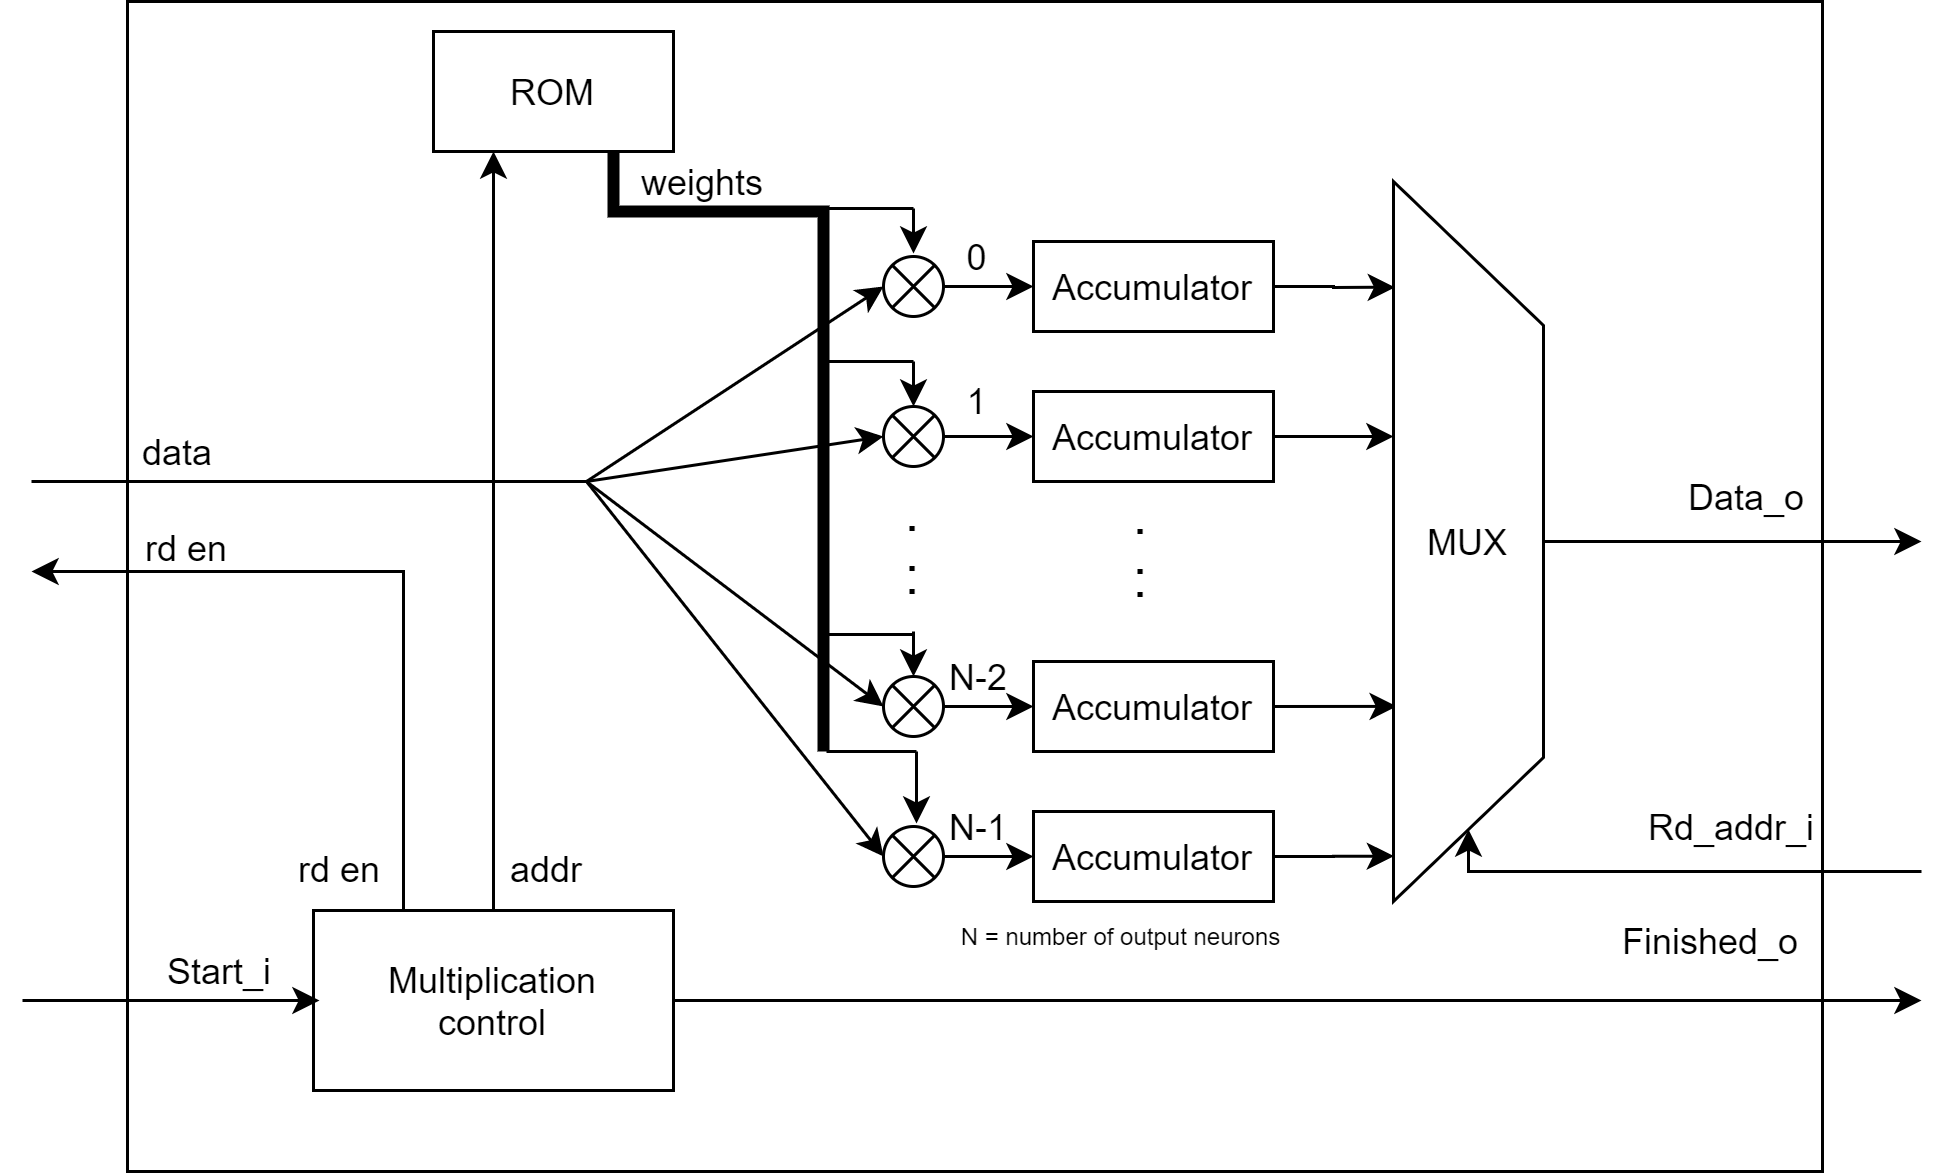
\includegraphics[width=1\textwidth]{img/blockDiagramDense.png}
	\caption[Dense layer diagram]{Dense layer diagram.}
	\label{FIG:denseLayerBlockDiagram}
\end{figure}


(Schematic is on figure \ref{FIG:denseLayerBlockDiagram}.)
This block contains a finite state machine. When the Start\_i input port goes high, input neurons are read from an external FIFO one by one. Each of the input neurons is multiplied by appropriate weight for each of the output neurons. These product are then fed to accumulators, which make a sum of all products of all neurons. When all of the incoming neurons are processed, the calculation is finished and a Finished\_o output port is raised high to signal that data is available.Result data can be addressed by Rd\_addr\_i port and read out at the Data\_o port.


Number of input neurons, output neurons and data width are generic. 

\subsubsection{Weights}

Weights are stored in a ROM memory. The values are hardcoded at synthesis. The VHDL code reads the weights from a file. File contains the weight values in binary. Each line represents all of the weights for one input neuron. There are as many lines as there are input neurons.

\subsubsection{Bias terms}

Bias terms are also loaded from a file. Each output neuron has its own bias term. Each line contains one bias term. Bias term bit width is generic. Bias terms are treated as a signed value.
	

\subsubsection{Parameters}
\begin{description}
	\item [VECTOR\_WIDTH   : integer] Bit width of input data.
	\item [INPUT\_COUNT    : integer] Number of input neurons
	\item [OUTPUT\_COUNT   : intege] Number of output neurons.
	\item [ROM\_FILE       : string] File, that holds the weight values.
	\item [BIAS\_WIDTH     : integer] Bit width of the bias terms.
	\item [BIAS\_FILE      : string] File, that holds the bias term values.
\end{description}


